\chapter{Feed Forward Neural Networks}

\begin{figure}[H]
	\centering
	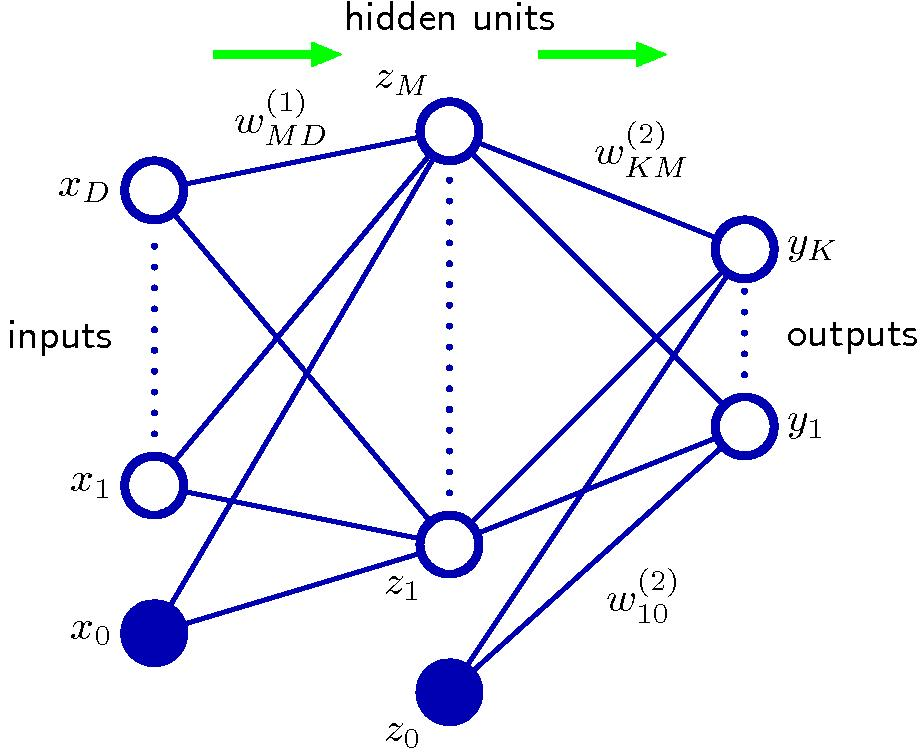
\includegraphics[width=0.5\linewidth]{ffnn_1}
	\caption{}
	\label{fig:ffnn1}
\end{figure}

\begin{figure}[H]
	\centering
	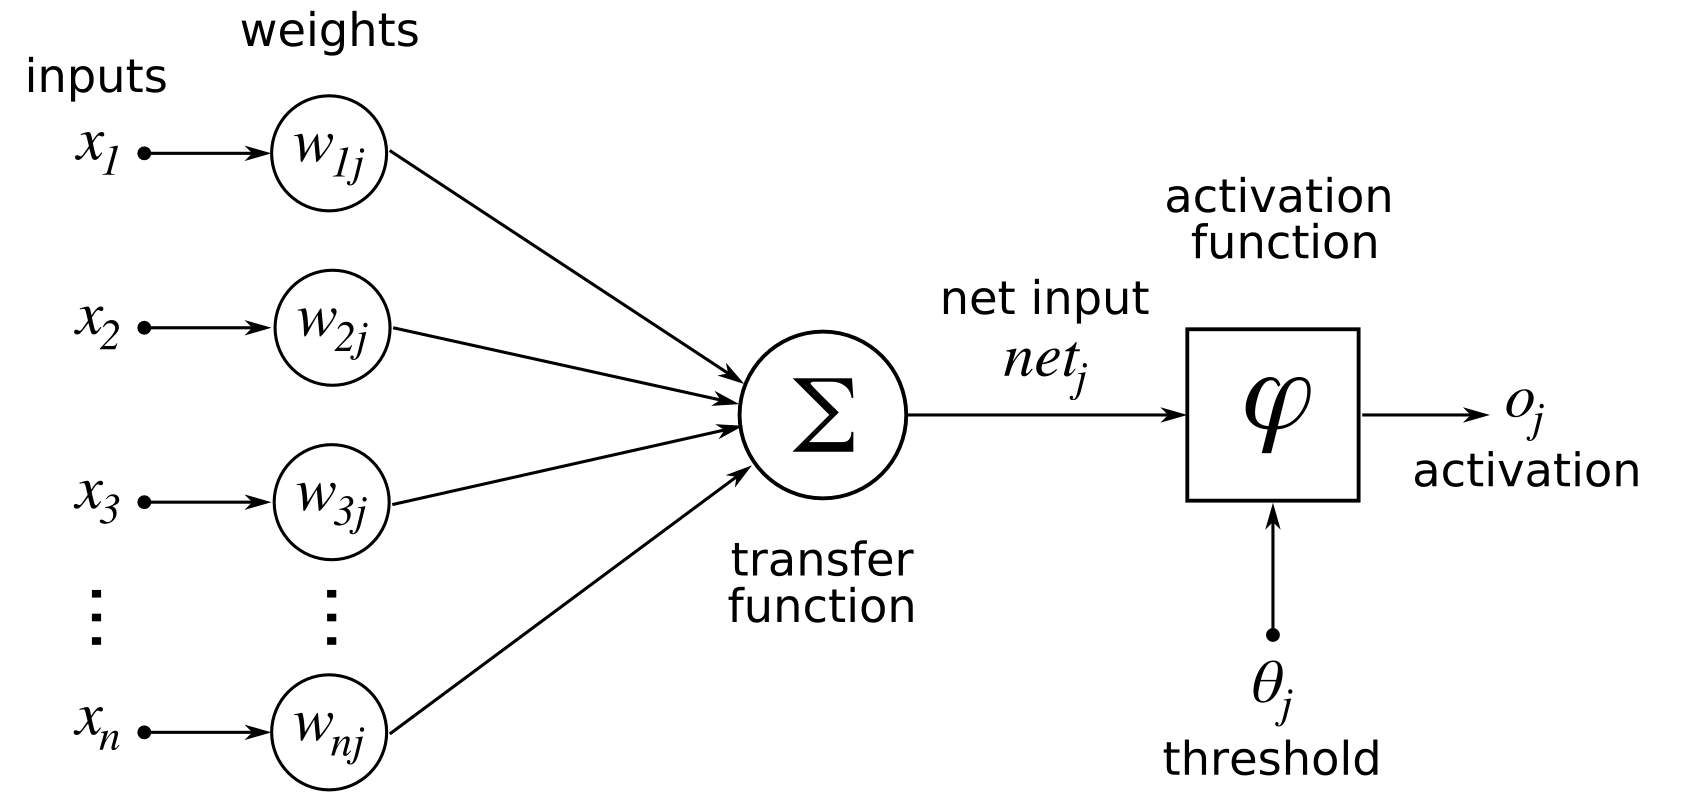
\includegraphics[width=0.6\linewidth]{ffnn_2}
	\caption{}
	\label{fig:ffnn2}
\end{figure}

Each layer first computes what is equivalent to the output $a_j$ of a linear statistical model and then applies a non-linear function to the linear model output. For the \textbf{first layer}, which takes the network input $x$ (that is a vector $x = (x_0,\ \dots,\ x_D)$) as input, these two steps look like this:

$$
\begin{aligned}
	a^{(1)}_j & = \sum_{i=1}^D w^{(1)}_{ji} x_i + w^{(1)}_{j0} \\
	z^{(1)}_j & = h_1(a^{(1)}_j )
\end{aligned}
$$

where $h_1$ is the non-linear (activation) function in the first layer. The superscript ${}^{(k)}$ indicates the index of the layer. \\
We can get rid of writing the so-called \textbf{bias} $w^{(1)}_{j0}$ explicitly by adding an extra input $x_0$ that is always set to one and extending the sum to go from zero:
$$
\begin{aligned}
	a^{(1)}_j & = \sum_{i=0}^D w^{(1)}_{ji} x_i 
\end{aligned}
$$
We will use this notation in the following for all layers and just write for example $\sum_i \ldots$ to be understood as $\sum_{i=0}^D \ldots$\\

The \textbf{second layer} takes the output the of the first layer as input:  
$$
a^{(2)}_j = \sum_{i}^M w^{(2)}_{ji} z^{(1)}_i 
$$
The second layer non-linear function is denoted by $h_2$ so the output of the network is
$$
y_j = h_2(a^{(2)}_j)
$$
This gives an example of how the neural network model input to output mapping can be specified. 

$$
h_2\left( \sum_{i}^M w^{(2)}_{ji} h_1 \left( \sum_{i=1}^D w^{(1)}_{ji} x_i + w^{(1)}_{j0} \right) \right)
$$